\documentclass{article}
\usepackage{qilin}
\title{ECE159 Notes}
\author{QiLin Xue}
\lhead{ECE159}
\rhead{QiLin Xue}
% % \renewcommand{\qedsymbol}{
\includegraphics[height=3ex]{kalda.png}}

\newcommand{\equals}{=}

\begin{document}
    \maketitle
    % The following notes were compiled from several sources: The majority of the theory was taken from the lectures and textbook, although some parts were taken from Purcell and Morin's \textit{Electricity and Magnetism}, and the problems were taken from Jaan Kalda's \href{https://www.ioc.ee/~kalda/ipho/electricity-circuits.pdf}{handout} on electrical circuits (hence the funky notation). Solutions were written as part of a joint \href{https://physoly.tech/kalda/}{collaboration}. I do not claim originality of the problems or solutions, though I selected them to reflect the course.
    \tableofcontents
    % \section{Positionality}
\begin{itemize}
    \item A \textbf{position} defines your orientation with respect to an \textbf{entity}.
    \begin{idea}
        How does PIAA affect positionality?
    \end{idea}
    Some ideas from classmates:
    \begin{itemize}
        \item Perception sets initial opinion
        \item You interpret things based on your positionWhat or what you don't perceive affects your positionality.
        \item In breaking the action of perceive-act, you include steps that allow the time to assess your position.
        \item Filters (in perception) depend on position
        \item Understanding your position allows you to assess your interpretations
    \end{itemize}
    \item Subconcious \textbf{bias} will be brought to the table depending on your position, so others can explicityl see how \textit{you} are looking at a situation. 
\end{itemize}
    \section{DC circuit Analysis}
    \subsection{Voltage and Current Division}
    For a series circuit, we can calculate the equivalent resistance by adding them.
    \begin{center}
        \begin{tikzpicture}[transform shape, thick]
            \draw (0, 0) to [V, i_>=$i$,
                                l=$V$, invert] (0, 4)
                         to [R, l=$R_1$] (4, 4) node[right] {$A$}
                         to [R, l=$R_2$] (4, 0)
                         to node[ground]{} (0,0); 
            \draw[fill=black] (4,4) circle (1.5pt);
            \draw[fill=black] (4,0) circle (1.5pt);
        \end{tikzpicture}
    \end{center}
    For this circuit, we have:
    \begin{equation}
        R_\text{eq} = R_1 + R_2
    \end{equation}
    and the voltage:
    \begin{equation}
        V_A = \frac{R_2}{R_1+R_2}V
    \end{equation}
    \begin{proof}
        The current is given by $i = \frac{V}{R_1+R_2}$ and the voltage at $A$ is given by:
        \begin{equation}
            V_A = V - iR_1 = V\left(1 - \frac{R_1}{R_1+R_2}\right) = \frac{R_2}{R_1+R_2}V
        \end{equation}
    \end{proof}
    For a parallel circuit, the effective resistance is the harmonic sum:
    \begin{center}
        \begin{tikzpicture}[transform shape, thick, american currents]
        \draw (0, 0) to [V, i_>=$i$, l=$V$] (0, 4)
                     -- (4,4)
                     to [R,i_>=$i_1$, l=$R_1$] (4, 0)
                     -- (0,0);
        \draw (4,4) -- (8,4)
                    to [R, i_>=$i_2$, l=$R_2$] (8,0)
                    to node[ground]{} (0,0);
        \end{tikzpicture}
    \end{center}
    In this circuit, we have:
    \begin{equation}
        R_\text{eq} = \left(\frac{1}{R_1} + \frac{1}{R_2}\right)^{-1} = \frac{R_1R_2}{R_1+R_2}
    \end{equation}
    and the current in the branches is given by:
    \begin{equation}
        i_1 = \frac{R_2}{R_1+R_2}i
    \end{equation}
    \begin{proof}
        The voltage drop across $R_1$ and $R_2$ must be the same, so:
        \begin{equation}
            i_1R_1 = i_2R_2
        \end{equation}
        We also have $i_2=i-i_1$, which gives:
        \begin{equation}
            i_1R_1 = (i-i_1)R_2 \implies i_1 = \frac{R_2}{R_1+R_2}i
        \end{equation}
    \end{proof}
    \subsection{Mesh Analysis}
    In mesh analysis, Kirchoff's Voltage law $\sum V = 0$ is written for each independent loop, and a system of equation is solved. The number of independent loops can be determined by finding the minimum number of wire cuts needed such that there are no loops.
    \begin{center}
        \begin{tikzpicture}[transform shape, thick, american currents]
        \draw (-4, 0) to [V, i_>=$i$, l_=$V\equals 2\si{\volt}$, invert] (4, 0)
                     -- (4,3) -- (3.5, 3) -- (3.5, 4) to
                [R, l_=$R_2\equals3\si{\ohm}$, i=$i-i_1$] (0,4) node[above] {$a$} to
                [R, l_=$R_1\equals 2\si{\ohm}$, i=$i-i_1+i_2$] (-3.5, 4)
                -- (-3.5, 3) -- (-4, 3) to node[ground,rotate=-90]{} (-4,0);
        \draw (-3.5, 3) -- (-3.5, 2) to [R, l_=$R_4\equals 5\si{\ohm}$, i<=$i_1-i_2$] (0,2) node[below] {$b$} to [R, l_=$R_5\equals 1\si{\ohm}$, i<=$i_1$] (3.5, 2) -- (3.5, 3);
        \draw (0, 4) to [R, l_=$R_3\equals 4\si{\ohm}$] (0,2);
        \draw (-2.5,3) node[scale=3]{$\circlearrowleft$} node{$A$};
        \draw (2,3) node[scale=3]{$\circlearrowleft$} node{$B$};
        \draw (0,1) node[scale=3]{$\circlearrowleft$} node{$C$};
        \end{tikzpicture}
    \end{center}
    We have three independent loops, labelled as $A,B,C$, which gives the system of three equations:
    \begin{align}
        0 &= -i_2R_3-(i-i_1+i_2)R_1+(i_1-i_2)R_4 \\ 
        0 &= -(i-i_1)R_2 + i_2R_3 + i_1R_5 \\ 
        0 &= V - i_1R_5 - (i_1-i_2)R_4
    \end{align}
    Solving this system gives:
    \begin{equation}
        (i, i_1, i_2) =\left(-\frac{144}{181}\si{A}, \frac{82}{181}\si{A}, \frac{26}{181}\si{A}\right)
    \end{equation}
    which can be used to determine the currents in all resistors and the associated voltages.
    \subsection{Nodal Analysis}
    In nodal analysis, we deal with the potentials at each node and write out Kirchoff's current law $\sum I = 0$ for the current \textit{leaving} (or alternatively, entering) each node for each node where the potential is unknown. Let the nodes labelled $a$ and $b$ have potentials $V_a$ and $V_b$. Then we have:
    \begin{align}
        0 &= \frac{V_a-V}{R_2} + \frac{V_a-V_b}{R_3} + \frac{V_a-0}{R_1} \\
        0 &= \frac{V_b-V}{R_5} + \frac{V_b-V_a}{R_3} + \frac{V_b-0}{R_4} 
    \end{align}
    which after solving, gives:
    \begin{equation}
        (V_a, V_b) = \left(\frac{176}{181}\si{V}, \frac{280}{181}\si{V}\right)
    \end{equation}
    which can be easily confirmed via the mesh analysis done above.
    \subsection{Superposition}
    Kirchoff's equations are linear. Each term includes only a first power of a current or a voltage, hence we can apply superposition. Let there be $n$ independent voltage sources and $m$ independent current sources. The current in the $j^\text{th}$ wire can be found as:
    \begin{equation}
        I_j = \sum_{k=1}^{n+m} I_j(k)
    \end{equation}
    where $I_j(k)$ is the current in that wire when only the $k^\text{th}$ battery (or current source) is included into the circuit. All other batteries are short circuited and all other current sources are removed by cutting off a connection wire.
    \begin{example}
        In the following circuit, we have $\mathcal{E}_1=\mathcal{E}_2$ and all the resistors are equal: $R_1=R_2=R_3=R_4=R$. Let us attempt to find the current through each resistor.
        \begin{center}
            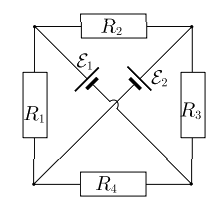
\includegraphics[width=0.3\linewidth]{estpho2012.png}
        \end{center}
        We make use of the superposition principle and start by short-circuiting $\mathcal{E}_2$. This leads to the following equivalent circuit:
    \begin{center}
        \begin{tikzpicture}[transform shape, thick]
        \ctikzset{bipoles/thickness=2}
        \ctikzset{label/align = smart}
        \coordinate  (A) at (0,0);
        \coordinate  (B) at (3,0);
        \coordinate  (C) at (6,0);
        \coordinate  (D) at (9,0);
        
        \draw (B) to [battery1, l=$\mathcal{E}_1$] (C) to ($(C) + (0,1)$) to [R, l=$R_3$] ($(D) + (0,1)$) to ($(D) + (0,-2)$) to ($(A) + (0,-2)$) to ($(A) + (0,1)$) to [R, l=$R_1$] ($(B) + (0,1)$) to (B);
        
        \draw ($(A) + (0,-1)$) to [R, l=$R_2$] ($(B) + (0,-1)$) to (B);
        \draw (C) to ($(C) + (0,-1)$) to [R, l=$R_4$] ($(D) + (0,-1)$);
        \end{tikzpicture}
        \end{center}
        Since all resistors have a resistance of $R$, this leads to the following currents in each resistor (going back to the original diagram):
        \begin{align*}
            R_1 &\rightarrow \frac{\mathcal{E}}{2R} \, \text{(downwards)} \\ 
            R_2 &\rightarrow \frac{\mathcal{E}}{2R} \, \text{(rightwards)} \\ 
            R_3 &\rightarrow \frac{\mathcal{E}}{2R} \, \text{(downwards)} \\
            R_4 &\rightarrow \frac{\mathcal{E}}{2R} \, \text{(leftwards)}
        \end{align*}
        and similarly if we short $\mathcal{E}_1$, we get the following currents:
        \begin{align*}
            R_1 &\rightarrow \frac{\mathcal{E}}{2R} \, \text{(downwards)} \\ 
            R_2 &\rightarrow \frac{\mathcal{E}}{2R} \, \text{(leftwards)} \\ 
            R_3 &\rightarrow \frac{\mathcal{E}}{2R} \, \text{(downwards)} \\
            R_4 &\rightarrow \frac{\mathcal{E}}{2R} \, \text{(rightwards)}
        \end{align*}
        By considering the superposition of these currents, we get after adding them together:
        \begin{align*}
            R_1 &\rightarrow \frac{\mathcal{E}}{R} \, \text{(downwards)} \\ 
            R_2 &\rightarrow 0 \\ 
            R_3 &\rightarrow \frac{\mathcal{E}}{R} \, \text{(downwards)} \\
            R_4 &\rightarrow 0
        \end{align*}
        Alternatively we can solve this problem via symmetry. Note that there is reflection symmetry across the vertical line. This means that the current does not have a preferred direction of going either right or left, so that the current in $R_2$ and $R_4$ will be zero. As a result, we can simply replace these two resistors with an open gap, which results in the other four circuit elements in series:
        $$    I = \frac{2\mathcal{E}}{2R} = \frac{\mathcal{E}}{R}
        $$
        which travels in a ``zigzag'' pattern.
    \end{example}
    
    \subsection{Source Transformation}
    A source transformation is the process of replacing a voltage source $v_s$ in series with a resistor $R$ by a current source $i_s$ in parallel with a resistor $R$, or vice versa. For example, these two circuits are equivalent:
    \begin{center}
        \begin{tikzpicture}[transform shape, thick]
            \draw (3,0) node[right] {$b$} -- (0, 0) to [V,
                                l=$v_s$, invert] (0, 2)
                         to [R, l=$R$] (3, 2) node[right] {$a$}; 
        \end{tikzpicture}
        \begin{tikzpicture}[transform shape, thick, american currents]
            \draw (3,0) node[right] {$b$} -- (0, 0) to [I,
                                l=$i_s$] (0, 2)
                         -- (3, 2) node[right] {$a$}; 
            \draw (1.5,0) to [R, l_=$R$] (1.5, 2);
        \end{tikzpicture}
    \end{center}
    where $v_s=i_sR$.
    \begin{proof}
        We can show that this is valid by letting $V_a=V$ and $V_b=0$. and calculating the current at $a$. For the first circuit, we have:
        \begin{equation}
            i = \frac{v_s-V}{R}
        \end{equation}
        For the second circuit, the current through the resistor is $i_R = \frac{V}{R}$ (downwards) and letting $i_s = \frac{v_s}{R}$ we have the current at $a$ as:
        \begin{equation}
            i = \frac{v_s}{R} - \frac{V}{R}
        \end{equation}
        which we see is the same for both cases.
    \end{proof}
    \begin{example}
        Suppose we have $n$ batteries with a voltage of $\mathcal{E}_i$ and internal resistances of $r_i$ with $i=1,2,\dots,n$, all connected in parallel. What is the effective electromotive force and the internal resistance of such a system of batteries?
        \vspace{2mm}

        We treat the batteries as $n$ current sources providing a current of $I_i = \dfrac{\mathcal{E}_i}{r_i}$. When determining an equivalent circuit, all the current sources add up to a total current of:
$$I_\text{total} = \sum_{i=1}^n \frac{\mathcal{E}_i}{r_i}$$and applying the idea again, this is equivalent to an effective voltage source of $\mathcal{E}_\text{eff} = I_\text{total}R_\text{eff}$ with the effective resistance being:
$$R_\text{eff} = \left(\sum_{i=1}^nr_i^{-1}\right)^{-1}$$since we are adding resistors in parallel. Putting everything together gives:
$$\mathcal{E}_\text{eff} = \left(\sum_{i=1}^nr_i^{-1}\right)^{-1}\sum_{i=1}^n \frac{\mathcal{E}_i}{r_i}$$
\end{example}
\subsection{Thevenin Equivalent Circuit}
Thevenin's Theorem tells us that any two-terminal circuit can be replaced by an equivalent voltage source $V_\text{th}$ in series with a resistor $R_\text{th}$. These are related via:
\begin{equation}
    \label{thevenin}
    R_\text{th} = \frac{V_\text{th}}{I_\text{sc}}
\end{equation} 
To calculate $V_\text{th}$, we find the \textit{open circuit} voltage between the two terminals. To calculate $R_\text{th}$, there are two options:
\begin{enumerate}
    \item Remove all independent voltage and current sources and calculate the equivalent resistance across the terminals.
    \item Connect the two terminals via a wire with negligible resistance. Calculate the current $I_\text{sc}$ through this wire and we can calculate $R_\text{th}$ using equation \ref{thevenin}.
\end{enumerate}
\begin{example}
    Take the following circuit. What is the maximal power which can be dissipated on a load connected to the leads of the circuit?
    \begin{center}
        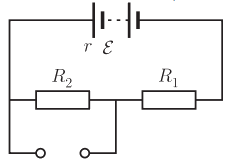
\includegraphics[width=0.3\linewidth]{pr10.png}
    \end{center}
    Recall that any circuit which consists of only resistors and batteries and has two ports $A$ and $B$ is equivalent to a series connection of a battery and a resistance. In other words, we consider the Thevenin equivalent of the circuit. The equivalent internal resistance can be found easily replacing the battery by a wire and using series and parallel connections.
$$R_{\text{eq}} = \frac{R_2(R_1+r)}{R_2 + (R_1+r)}$$The equivalent emf $\mathcal{E}_{\text{eq}}$ is the potential drop across $R_2$. The net resistance about the battery is $R_2 + (R_1+r)$, so the current through the battery is ,
\[ I = \mathcal{E}/r\implies I = \frac{\mathcal{E}}{R_1+R_2+r}.\]The potential drop about $R_2$ is then
\[V = IR_2 = \mathcal{E}\frac{R_2}{R_1+R_2+r}.\]This means that entire circuit in the figure can be substituted with an equivalent battery with
$$\mathcal{E}_{\text{eq}} = \mathcal{E}\frac{R_2}{R_1+R_2+r}.$$By the maximal power transfer theorem, this means that the resistance of the load attached needs to be $R=R_\text{eq}$. The potential drop across it is $\frac{\mathcal{E}}{2}$, so we have: 
\begin{align*}
P_{\text{max}} = \frac{\mathcal{E}_{\text{eq}}^2}{4R_{\text{eq}}} &= \frac{1}{4}\mathcal{E}^2 \left(\frac{R_2}{R_1+R_2+r}\right)^2 \cdot \frac{R_2 + (R_1+r)}{R_2\times (R_1+r)} \\
&= \frac{1}{4}\frac{R_2}{(r + R_1 + R_2)(R_1 + r)}\mathcal{E}^2
\end{align*}
\end{example}
\subsection{Norton Equivalent Circuit}
Similar to Thevenin, we can also perform a source transformation such that we can replace any subcircuit element with an independent current source connected to a resistor in parallel. Note that calculating the equivalent resistance is done in the same way.
\section{Operational Amplifiers}
An operational amplifier (op amp) is an active circuit element designed to perform mathematical operations of addition, subtraction, multiplication, division, differentiation, and integration.
\begin{center}
    \begin{circuitikz}[line width=1pt]
        \draw
        (0,0) node[op amp,yscale=1](opamp){} 
        (opamp.+) to[short, -o] ++(-.5,0) node[left]{$v_2$}
        (opamp.-) to[short, -o] ++ (-.5,0) node[left]{$v_1$}
        (opamp.out) to[short, -o] ++ (.5,0) node[right]{$v_0$}
        ;
    \end{circuitikz}
    
\end{center}
It is equivalent to the following circuit:
\begin{center}
    \begin{tikzpicture}[transform shape, thick]
        \draw  (-2,2) to [short, -o] (-2,2) node[left] {$v_1$} -- (0, 2) to [R, l=$R_i$, v_<=$v_d$] (0,-2) to [short, -o] (-2,-2) node[left] {$v_2$};

        \draw (6,0) node[right] {$v_0$} to [short, -o] (6,0) to [R, l=$R_0$] (3,0) to [V, l_=$A(v_2-v_1)$] (3, -1.5) node[ground]{};
    \end{tikzpicture}
\end{center}
where $A \gg 1$ is known as the open-loop voltage gain. The input resistance $R_i$ is typically very big.
\subsection{Ideal OP Amp}
For an ideal OP Amp, we have an infinite open-loop gain, infinite input resistance, and zero output resistance. This gives the following results:
\begin{itemize}
    \item The currents into both input terminals are zero.
    \item Voltage across input terminals are zero.
\end{itemize}
\begin{example}
    Suppose we have the OP Amp circuit and we wish to find $v_0$
    \begin{center}
        \begin{tikzpicture}[transform shape, thick]
            \draw (7.25,0) to [short, -o] (7.25,0) -- (0,0) to [V, l=$v_s\equals 2\si{\volt}$, invert] (0,3) to [R, l=$10\si{\kilo\ohm}$] (3,3);

            \draw
            (5,2.5) node[op amp,yscale=1](opamp){} 
            (opamp.+) to ++ (-0.5,0) to ++ (0, -2) node[ground]{}
            (opamp.-) -- (3,3)
            (opamp.out) to[short, -o] ++ (1,0) node[right] {$v_0$};
            
            \draw (3,3) -- (3,4) to [R, l=$20\si{\kilo\ohm}$] (6.5,4) -- (6.5,2.5);
        \end{tikzpicture}
    \end{center}
    Since the terminals ahve equal voltage, and the positive end is connected to the ground, then we must have:
    \begin{equation*}
        2V - i(10\si{\kilo\ohm}) = 0 \implies i = 0.2\si{\milli\ampere}
    \end{equation*}
    and thus:
    \begin{equation*}
        v_0 = -i\cdot 20\si{\kilo\ohm} = -4\si{\volt}
    \end{equation*}
    This is known as an \textbf{inverting amplifier}.
\end{example}
\subsection{Types of Amplifiers}
Here is a list of common amplifiers:
\begin{itemize}
    \item Inverting Amplifier:
    \begin{equation}
        v_0 = -\frac{R_2}{R_1} v_i
    \end{equation}
    \begin{center}
        \begin{tikzpicture}[transform shape, thick]
            \draw (0,3) node[left] {$v_i$} to [short, -o] (0,3) to [R, l=$R_1$] (3,3);

            \draw
            (5,2.5) node[op amp,yscale=1](opamp){} 
            (opamp.+) to ++ (-0.5,0) to ++ (0, -2) node[ground]{}
            (opamp.-) -- (3,3)
            (opamp.out) to[short, -o] ++ (1,0) node[right] {$v_0$};
            
            \draw (3,3) -- (3,4) to [R, l=$R_2$] (6.5,4) -- (6.5,2.5);
        \end{tikzpicture}
    \end{center}
    \item Noninverting amplifier:
    \begin{equation}
        v_0 = \left(1+\frac{R_2}{R_1}\right)v_i
    \end{equation}
    \begin{center}
        \begin{tikzpicture}[transform shape, thick]
            \draw (0,3) node[ground] {} to [R, l=$R_1$] (3,3);

            \draw
            (5,2.5) node[op amp,yscale=1](opamp){} 
            (opamp.+) to[short,-o] ++ (-0.5,0) node[left] {$v_i$}
            (opamp.-) -- (3,3)
            (opamp.out) to[short, -o] ++ (1,0) node[right] {$v_0$};
            
            \draw (3,3) -- (3,4) to [R, l=$R_2$] (6.5,4) -- (6.5,2.5);
        \end{tikzpicture}
    \end{center}
    \item Voltage follower:
    \begin{equation}
        v_0 = v_i
    \end{equation}
    \begin{center}
        \begin{tikzpicture}[transform shape, thick]

            \draw
            (5,2.5) node[op amp,yscale=1](opamp){} 
            (opamp.+) to[short,-o] ++ (-0.5,0) node[left] {$v_i$}
            (opamp.-) -- (3,3)
            (opamp.out) to[short, -o] ++ (1,0) node[right] {$v_0$};
            
            \draw (3,3) -- (3,4) -- (6.5,4) -- (6.5,2.5);
        \end{tikzpicture}
    \end{center}
    \item Summer:
    \begin{equation}
        v_0 = -\left(\frac{R_f}{R_i}v_1 + \frac{R_f}{R_2}v_2 + \frac{R_f}{R_3}v_3\right)
    \end{equation}
    \begin{center}
        \begin{tikzpicture}[transform shape, thick]
            \draw (0,3) node[left] {$v_2$} to[short, -o] (0,3) to [R, l=$R_2$] (2,3) -- (3,3);
            \draw (0,4) node[left] {$v_1$} to[short, -o] (0,4) to [R, l=$R_1$] (2,4) -- (2,3);
            \draw (0,2) node[left] {$v_3$} to[short, -o] (0,2) to [R, l=$R_3$] (2,2) -- (2,3);

            \draw
            (5,2.5) node[op amp,yscale=1](opamp){} 
            (opamp.+) to ++ (-0.5,0) to ++ (0, -2) node[ground]{}
            (opamp.-) -- (3,3)
            (opamp.out) to[short, -o] ++ (1,0) node[right] {$v_0$};
            
            \draw (3,3) -- (3,4) to [R, l=$R_f$] (6.5,4) -- (6.5,2.5);
        \end{tikzpicture}
    \end{center}
    \item Difference Amplifier:
    \begin{equation}
        v_0 = \frac{R_2}{R_1}(v_2-v_1)
    \end{equation}
    \begin{center}
        \begin{tikzpicture}[transform shape, thick]
            % \draw (0,3) node[left] {$v_2$} to[short, -o] (0,3) to [R, l=$R_2$] (2,3) -- (3,3);
            % \draw (0,4) node[left] {$v_1$} to[short, -o] (0,4) to [R, l=$R_1$] (2,4) -- (2,3);
            % \draw (0,2) node[left] {$v_3$} to[short, -o] (0,2) to [R, l=$R_3$] (2,2) -- (2,3);

            \draw
            (5,2.5) node[op amp,yscale=1](opamp){} 
            (opamp.+) to ++ (-0.5,0) to ++ (0, -1) to [R, l=$R_2$] (6.5, 1) node[ground] {}
            (opamp.-) to ++ (-0.5,0) to ++ (0,1) to [R, l=$R_2$] (6.5,4) -- (6.5,2.5)
            (opamp.out) to[short, -o] ++ (1,0) node[right] {$v_0$};
            
            \draw (0,4) node[left] {$v_1$} to [short, -o] (0,4) to [R, l=$R_1$] (3.29,4);
            \draw (0,1) node[left] {$v_2$} to [short, -o] (0,1) to [R, l=$R_1$] (3.29,1);

        \end{tikzpicture}
    \end{center}
\end{itemize}
\section{First Order Circuits}
\subsection{Capacitors and Inductors}
A capacitor is able to store charge such that the voltage across it is:
\begin{equation}
    V = \frac{q}{C}
\end{equation}
where $C$ is the capacitance. Differentiating both sides, we have:
\begin{equation}
    \frac{dV}{dt} = \frac{i}{C} \implies i = C\frac{dV}{dt}
\end{equation}
Since the current cannot be infinite, the voltage across a capacitor must be differentiable (i.e. smooth). When multiple capacitors are in series, the equivalent capacitance is:
\begin{equation}
    C_\text{eq} = \left(\frac{1}{C_1}+\frac{1}{C_2} + \cdots\right)^{-1}
\end{equation}
For multiple capacitors in parallel, the equivalent capacitance is:
\begin{equation}
    C_\text{eq} = C_1+C_2+\cdots
\end{equation}
The energy stored in a capacitor is given by:
\begin{equation}
    U = \frac{q^2}{2C} = \frac{1}{2}CV^2 = \frac{q}{2V}
\end{equation}
An inductor maintains a voltage that resists a change in current (i.e. via Lenz's Law). This means the voltage across a resistor is:
\begin{equation}
    V = -L\frac{di}{dt}
\end{equation}
where $L$ is the inductance. Since the voltage across cannot be infinite, the current across it has to be differentiable. When inductors are added in series, the equivalent inductance is:
\begin{equation}
    L_\text{eq} = L_1 + L_2 + \cdots
\end{equation}
and in parallel:
\begin{equation}
    L_\text{eq} = \left(\frac{1}{L_1} + \frac{1}{L_2}+\cdots\right)^{-1}
\end{equation}
The energy stored in an inductor is:
\begin{equation}
    U = \frac{1}{2}Li^2
\end{equation}
\begin{idea}
    For $RL$ and $RC$ circuits, at time scales much shorter than the characteristic times $\tau = RC$ or $\tau = L/R$ (i.e. right after a switch is opened), the capacitor's charge and inductor's current remain almost constant. In particular, if a capacitor was chargeless, its voltage remains almost zero (i.e. short circuit). If there was no current in an inductor, its current remains zero (i.e. inductor may be considered to be broken). If a capacitor had a charge $Q$ corresponding to a voltage $V_0$, its voltage remains essentially constant (i.e. it acts and can be substituted by a battery of voltage $V$). Similarly, if an inductor had a current $I_0$, it can be substituted by a respective constant current source. If we try to forcefully break the current through an inductor by switching it off, a rapid fall of current $I$ creates a huge voltage $-L\frac{dI}{dt}$ which usually leads to a spark at the switch.
    \vspace{2mm}

    At time scales much larger than the characteristic times, the situation is reversed: the inductor can be considered a short-circuiting wire, and capacitor as an insulator. This is because all the currents and voltages tend exponentially towards the equilibrium state so that the different from the equilibrium value $\Delta \propto e^{-t/\tau}$: the capacitor charge is almost constant, hence there is no current, and the inductor current is almost constant, hence no voltage.
\end{idea}
\subsection{Natural Response}
Since resistors provide a ``decaying response'' (see the mechanical analogy section), it is expected that RC and RL circuits have a decaying exponential, when there are no voltage sources:
\begin{equation}
    x(t) = x(0)e^{-t/\tau}
\end{equation}
where $x(0)$ is the initial value of a quantity (current or voltage), and $\tau$ is the time constant. For RC circuits, we have $\tau = RC$ and for RL circuits, we have $\tau = L/R$. It is the characteristic time for which a certain quantity decreases by a factor of $\frac{1}{e}$. For an $RC$ circuit, we can derive this from the equation:
\begin{equation}
    i_c + i_r = 0 \implies C\frac{dV}{dt} + \frac{V}{r} = 0
\end{equation}
though I prefer working with Kirchoff's Voltage Law:
\begin{equation}
    -\frac{dq}{dt}R - \frac{q}{C} = 0
\end{equation}
This is because we see a similar structure for the inductor:
\begin{equation}
    -iR - L\frac{di}{dt} = 0
\end{equation}
Notice the connection between $q$, $i$, and $\frac{di}{dt}$. This is important when formulating the mathematics behind complex AC circuits later.
\subsection{Step Responses}
When we have a sudden change (i.e. a voltage or current source is added), the circuit may behave slightly differently. Since it is a first order circuit, we should still expect an exponential pattern. If we add a constant voltage or current term to the differential equation above, we can easily solve for it. Alternatively, we can abuse the fact that it is a linear differential equation so we can write the general solution as:
\begin{equation}
    \text{complete response} = \text{natural response} + \text{forced response} 
\end{equation}
or
\begin{equation}
    v = v_n + v_f
\end{equation}
or:
\begin{equation}
    v = v_t + v_{ss}
\end{equation}
Here, $v_t$ is the transient response, and it will die out with time. The steady state response $v_{ss}$ is the behaviour of the circuit a long time after an external excitation is applied. As a result, we can write out the voltage:
\begin{equation}
    v(t) = v(\infty) + [v(0)-v(\infty)]e^{-t/\tau}
\end{equation}
and similarly for an RL circuit:
\begin{equation}
    i(t) = i(\infty) + [i(0) -i(\infty)]e^{-t/\tau}
\end{equation}
\subsection{A Mechanical Analogy}
Consider a very light mechanical ball. We can make the following analogies:
\begin{itemize}
    \item charge ($q$ - displacement ($\Delta x$)
    \item voltage $V$ - force ($F$)
    \item capacitance $C$ - inverse spring constant ($1/k$)
    \item inductance $M$ - extra mass $M$
    \item resistor $R$ - damping constant $b$
    \item current $i$ - velocity $v$
    \item change in current $\frac{di}{dt}$ - acceleration $a$
\end{itemize}
If the current is not changing, then we can view the ball to be in equilibrium (i.e. $\sum F = 0$). While this gives intuition for more difficult circuits, it is also important to note that this is \textit{exactly equivalent}. For example, Nikita Sopenko (who is currently a grad student at CalTech) used this principle to solve the \href{https://www.ipho2012.ee/physicscup/problem-no-5/solution/}{fifth problem} of Physics Cup back in 2012.
\subsubsection*{Voltage Source + Resistor}
For a voltage source and resistor, we have the mechanical relationship of a mechanism supplying a force $F$ to the ball, and there is an opposing force (that comes from air resistance) of $-bv$. Therefore:
\begin{equation}
    F = bv
\end{equation}
which is equivalent to Ohm's law.
\subsubsection*{RC Circuit}
Suppose we have a capacitor $C$ that is initially charged, connected to a resistor $R$. Our mechanical analogy then becomes a light object connected to a spring. The spring wishes to pull the object towards equilibrium, but air resistance slows it down. Since the mass is zero, the net force is zero, so we have $kx=bv$. This means that as $x\to 0$, we will also have $v\to 0$, which results in an exponential decay behaviour.
\subsubsection*{RL Circuit}
Suppose we have an inductor (that initially has a current passing through it) connected in series with a resistor. This is equivalent to throwing a mass $M$ (without gravity) with a speed $v$ in the presence of air resistance. Intuitively, we know that this will give an exponential decay behaviour.
\subsubsection*{LC Circuits}
Suppose we have an inductor (with a current through it) connected to a capacitor (that is initially charged). Without working out the math, we know that this is equivalent to a ball of mass $M$ connected to a spring. This gives rise to simple harmonic motion, so we should expect a similar pattern in the current and voltage.
\subsubsection*{RLC Circuits}
Similar to the LC circuit, we have a ball of mass $M$ on a spring. However, there is now air resistance, so we should expect a decaying sinusoidal pattern.
\end{document}

